\chapter{Probability and Random Vectors}
\label{ch:prob}

\begin{objectives}
\begin{itemize}
  \item Build probability from its axioms: conditional probability, independence and Bayes' rule.
  \item Work with random variables and random vectors: densities, expectations, covariances and changes of variables.
  \item Derive the Gaussian distribution and its key properties: affine maps, marginals, conditionals and the fusion of estimates.
  \item Understand the law of large numbers, the central limit theorem and Monte Carlo methods.
  \item Derive the $\chi^2$ distribution and use it for hypothesis tests, the basis of gating and consistency checks.
  \item Understand how nonlinear functions distort distributions, and what linearization keeps and loses.
\end{itemize}
\end{objectives}

A filter does not merely estimate the state; it maintains a probability distribution over it. The estimate is the center of
that distribution, and the covariance describes its spread. This chapter develops the probability theory that gives these words a
precise meaning.

% ==============================================================================
\section{Probability}

\subsection{Events and the axioms}

A random experiment has a set $\Omega$ of possible outcomes, the \term{sample space}. An \term{event} is a subset of outcomes, and a
\term{probability} assigns to each event $A$ a number $P(A)$ obeying three axioms (Kolmogorov):
\begin{enumerate}
  \item $P(A) \ge 0$ for every event;
  \item $P(\Omega) = 1$;
  \item if $A_1, A_2, \dots$ are mutually exclusive (pairwise disjoint), $P(A_1\cup A_2\cup\cdots) = \sum_iP(A_i)$.
\end{enumerate}
Everything else follows: $P(\text{not }A) = 1 - P(A)$, $P(A\cup B) = P(A) + P(B) - P(A\cap B)$, and so on. Probability can be read as a
long-run frequency (the fraction of repetitions in which $A$ occurs) or as a degree of belief; the mathematics is the same, and filters
use both readings.

\subsection{Conditional probability and independence}

\begin{definition}[Conditional probability]
For $P(B) > 0$, the probability of $A$ given $B$ is $P(A\mid B) = P(A\cap B)/P(B)$.
\end{definition}

Conditioning restricts attention to the outcomes in which $B$ happened and renormalizes. Two events are \term{independent} if
$P(A\cap B) = P(A)P(B)$, equivalently $P(A\mid B) = P(A)$: knowing that $B$ occurred tells nothing about $A$.

\begin{proposition}[Law of total probability and Bayes' rule]
\index{Bayes' rule}
If $B_1, \dots, B_n$ are mutually exclusive and cover $\Omega$, then $P(A) = \sum_iP(A\mid B_i)P(B_i)$, and
\begin{equation}
  P(B_i\mid A) = \frac{P(A\mid B_i)\,P(B_i)}{\sum_jP(A\mid B_j)\,P(B_j)} .
\end{equation}
\end{proposition}
\begin{proof}
$A$ is the disjoint union of the $A\cap B_i$, and $P(A\cap B_i) = P(A\mid B_i)P(B_i)$. Bayes' rule is the definition of conditional
probability applied twice: $P(B_i\mid A)P(A) = P(A\cap B_i) = P(A\mid B_i)P(B_i)$.
\end{proof}

Bayes' rule turns the probability of an observation given a hypothesis (which a sensor model provides) into the probability of the
hypothesis given the observation (which we want).

\begin{worked}[how informative is a passed test?]
Suppose 10\% of the feature tracks reaching an outlier test are wrong. The test rejects 90\% of wrong tracks, and (being a 95\% gate)
also rejects 5\% of correct ones. A track passes. What is the probability that it is wrong? With $W$ = ``wrong'' and $A$ = ``passes'':
$P(A\mid W) = 0.1$, $P(W) = 0.1$, $P(A\mid\text{correct}) = 0.95$, $P(\text{correct}) = 0.9$. Bayes' rule gives
\begin{equation*}
  P(W\mid A) = \frac{0.1\times0.1}{0.1\times0.1 + 0.95\times0.9} = \frac{0.01}{0.865} \approx 1.2\% .
\end{equation*}
The test reduces the outlier fraction from 10\% to about 1\%: very useful, but not perfect, which is why the estimator adds further
checks downstream.
\end{worked}

% ==============================================================================
\section{Random variables}

\subsection{Distributions, densities and expectations}

A \term{random variable} $X$ is a numerical quantity determined by the outcome of an experiment. Its \emph{cumulative distribution
function} is $F(x) = P(X \le x)$. A discrete random variable takes countably many values with probabilities $p(x) = P(X = x)$; a continuous
one has a \term{probability density function} (pdf) $p(x) \ge 0$ with
\begin{equation}
  P(a \le X \le b) = \int_a^bp(x)\,\dd x, \qquad \int_{-\infty}^\infty p(x)\,\dd x = 1 .
\end{equation}
A density is not a probability: $p(x)\,\dd x$ is the probability of falling in a small interval of width $\dd x$ around $x$, and a density
can exceed one.

\begin{definition}[Expectation and variance]
The \term{expectation} (mean) of $X$ is $\E[X] = \int x\,p(x)\,\dd x$ (a sum for discrete variables). The expectation of a function of $X$ is
$\E[g(X)] = \int g(x)p(x)\,\dd x$. The \term{variance} is $\Var(X) = \E[(X - \E X)^2] = \E[X^2] - (\E X)^2$, and its square root is the
\term{standard deviation} $\sigma$.
\end{definition}

Expectation is linear: $\E[aX + bY + c] = a\E[X] + b\E[Y] + c$ for any random variables, dependent or not. Variance scales quadratically and
ignores shifts: $\Var(aX + c) = a^2\Var(X)$. The standard deviation has the units of $X$ and measures its typical spread.

\begin{example}[Uniform distribution]
$X$ uniform on $[a, b]$ has $p(x) = 1/(b - a)$ there, mean $(a + b)/2$ and variance $(b - a)^2/12$. Rounding a reading to a resolution
$\Delta$ produces an error that is approximately uniform on $[-\Delta/2, \Delta/2]$, with standard deviation $\Delta/\sqrt{12}$: the
quantization noise of a sensor.
\end{example}

\subsection{The Gaussian distribution}

\begin{definition}[Gaussian distribution]
\index{Gaussian distribution}
$X \sim \N(\mu, \sigma^2)$ has density
\begin{equation}
  p(x) = \frac{1}{\sqrt{2\pi}\,\sigma}\exp\!\Big(-\frac{(x - \mu)^2}{2\sigma^2}\Big).
\end{equation}
The \emph{standard normal} distribution is $\N(0, 1)$.
\end{definition}

\begin{proposition}[Normalization]
$\int_{-\infty}^\infty e^{-x^2/2}\,\dd x = \sqrt{2\pi}$.
\end{proposition}
\begin{proof}
Let $I$ be the integral. Then $I^2 = \iint e^{-(x^2 + y^2)/2}\,\dd x\,\dd y$. In polar coordinates, with area element $r\,\dd r\,\dd\theta$,
$I^2 = \int_0^{2\pi}\!\int_0^\infty e^{-r^2/2}r\,\dd r\,\dd\theta = 2\pi\big[-e^{-r^2/2}\big]_0^\infty = 2\pi$.
\end{proof}

Substituting $x \to (x - \mu)/\sigma$ shows that the general density integrates to one, and similar integrals (using symmetry and
integration by parts) give $\E[X] = \mu$ and $\Var(X) = \sigma^2$. If $X \sim \N(\mu, \sigma^2)$ then $(X - \mu)/\sigma \sim \N(0, 1)$, and the
probabilities of falling within one, two and three standard deviations of the mean are $68.27\%$, $95.45\%$ and $99.73\%$. A Gaussian is
completely determined by its mean and variance, and is closed under the operations a linear filter performs, which is why Kalman
filters can work with means and covariances alone.

% ==============================================================================
\section{Several random variables}

\subsection{Joint, marginal and conditional densities}

Two random variables $X, Y$ have a \emph{joint density} $p(x, y)$, with $P((X, Y) \in A) = \iint_Ap(x, y)\,\dd x\,\dd y$. From it:
\begin{align}
  \text{marginal:}&\quad p(x) = \int p(x, y)\,\dd y, \\
  \text{conditional:}&\quad p(x\mid y) = \frac{p(x, y)}{p(y)}, \\
  \text{Bayes' rule:}&\quad p(x\mid y) = \frac{p(y\mid x)\,p(x)}{p(y)} = \frac{p(y\mid x)\,p(x)}{\int p(y\mid x')p(x')\,\dd x'} .
\end{align}
$X$ and $Y$ are independent if $p(x, y) = p(x)p(y)$. In estimation, $x$ is the unknown state and $y$ the measurement: $p(y\mid x)$ is the
sensor model (the \emph{likelihood}), $p(x)$ is the \emph{prior}, and $p(x\mid y)$ the \emph{posterior}.

\subsection{Covariance and correlation}

The \term{covariance} $\Cov(X, Y) = \E[(X - \E X)(Y - \E Y)]$ measures how two variables vary together, and the \term{correlation
coefficient} $\rho = \Cov(X, Y)/(\sigma_X\sigma_Y) \in [-1, 1]$ normalizes it (the bound is the Cauchy--Schwarz inequality). Independent
variables have zero covariance, and then $\Var(X + Y) = \Var(X) + \Var(Y)$: variances of independent errors add.

The converse fails: zero correlation does not imply independence. If $X \sim \N(0, 1)$ and $Y = X^2$, then $\Cov(X, Y) = \E[X^3] = 0$, yet $Y$
is a function of $X$. Correlation measures only \emph{linear} dependence. (For jointly Gaussian variables the converse does hold, as shown
below.)

% ==============================================================================
\section{Random vectors}

\subsection{Mean and covariance}

For a random vector $x \in \R^n$ with density $p(x)$, the mean and \term{covariance matrix} are
\begin{equation}
  \mu = \E[x], \qquad \Sigma = \Cov(x) = \E\big[(x - \mu)(x - \mu)\T\big] = \E[xx\T] - \mu\mu\T .
\end{equation}
The diagonal of $\Sigma$ holds the variances $\sigma_i^2$ and its off-diagonal entries the covariances. $\Sigma$ is symmetric and positive
semi-definite: for any fixed $a$, $a\T\Sigma a = \E\big[(a\T(x - \mu))^2\big] \ge 0$. The \emph{cross-covariance} of two random vectors is
$\Sigma_{xy} = \E[(x - \mu_x)(y - \mu_y)\T]$, and $\Sigma_{yx} = \Sigma_{xy}\T$.

\begin{proposition}[Affine transformations]
\label{prop:affine}
If $y = Ax + b$ then $\E[y] = A\mu + b$ and $\Cov(y) = A\Sigma A\T$. If $x$ and $w$ are uncorrelated, $\Cov(Ax + Bw) = A\Sigma_xA\T + B\Sigma_wB\T$.
\end{proposition}
\begin{proof}
Linearity of expectation gives the mean. Then $\Cov(y) = \E[A(x - \mu)(x - \mu)\T A\T] = A\Sigma A\T$. With uncorrelated $x$ and $w$, the cross terms
$A\Sigma_{xw}B\T$ vanish.
\end{proof}

This one proposition is the covariance propagation of the Kalman filter ($P \leftarrow \Phi P \Phi\T + Q$), the covariance of a stacked
measurement, and the augmentation formula of stochastic cloning ($P \leftarrow JPJ\T$).

\begin{proposition}[Expected value of a quadratic form]
\label{prop:quadratic-expectation}
For any matrix $A$, $\E[x\T Ax] = \tr(A\Sigma) + \mu\T A\mu$. In particular, if $\mu = 0$ then $\E[x\T\Sigma\inv x] = \tr(I_n) = n$.
\end{proposition}
\begin{proof}
$x\T Ax = \tr(Axx\T)$, and expectation commutes with the trace: $\E[x\T Ax] = \tr(A\,\E[xx\T]) = \tr(A(\Sigma + \mu\mu\T))$.
\end{proof}

The special case is the reason a consistent filter's normalized estimation error squared averages to the dimension of the state
(\cref{ch:consistency}).

\subsection{Changing variables}

\begin{proposition}[Change of variables]
\label{prop:change-of-variables}
If $y = g(x)$ with $g$ invertible and differentiable, the densities are related by
$p_y(y) = p_x\big(g\inv(y)\big)\,\big|\det\frac{\partial g\inv}{\partial y}\big|$.
\end{proposition}

In one dimension this follows from equating probabilities of corresponding small intervals, $p_y(y)\,|\dd y| = p_x(x)\,|\dd x|$; in several
dimensions the determinant measures how $g\inv$ stretches volumes (\cref{sec:determinants}). For an invertible linear map $y = Ax$ the factor
is the constant $1/|\det A|$.

% ==============================================================================
\section{The multivariate Gaussian}

\subsection{Definition}

\begin{definition}[Multivariate Gaussian]
\index{Gaussian distribution!multivariate}
A random vector $x \in \R^n$ is Gaussian, $x \sim \N(\mu, \Sigma)$, if it can be written as $x = \mu + Ls$ where $s$ has independent standard
normal components and $LL\T = \Sigma$. If $\Sigma \succ 0$ its density is
\begin{equation}
  p(x) = \frac{1}{\sqrt{(2\pi)^n \det\Sigma}}\exp\!\Big( -\tfrac12 (x - \mu)\T \Sigma\inv (x - \mu) \Big).
  \label{eq:gaussian-pdf}
\end{equation}
The quantity $d_M^2(x) = (x - \mu)\T\Sigma\inv(x - \mu)$ is the squared \term{Mahalanobis distance} of $x$ from the mean.
\end{definition}

\begin{proof}[Derivation of the density]
The density of $s$ is the product of $n$ standard normal densities, $(2\pi)^{-n/2}\exp(-\tfrac12s\T s)$. By \cref{prop:change-of-variables} with
$s = L\inv(x - \mu)$, $p(x) = (2\pi)^{-n/2}\exp\big(-\tfrac12(x - \mu)\T L\mT L\inv(x - \mu)\big)/|\det L|$. Since $L\mT L\inv = (LL\T)\inv = \Sigma\inv$ and
$|\det L| = \sqrt{\det\Sigma}$, this is \eqref{eq:gaussian-pdf}.
\end{proof}

By \cref{prop:affine}, the mean of $x$ is $\mu$ and its covariance is $L\,\E[ss\T]L\T = \Sigma$. The definition also handles singular
covariances (with $L$ not invertible), which arise naturally in stochastic cloning (\cref{ch:cloning}).

\begin{figure}[t]
  \centering
  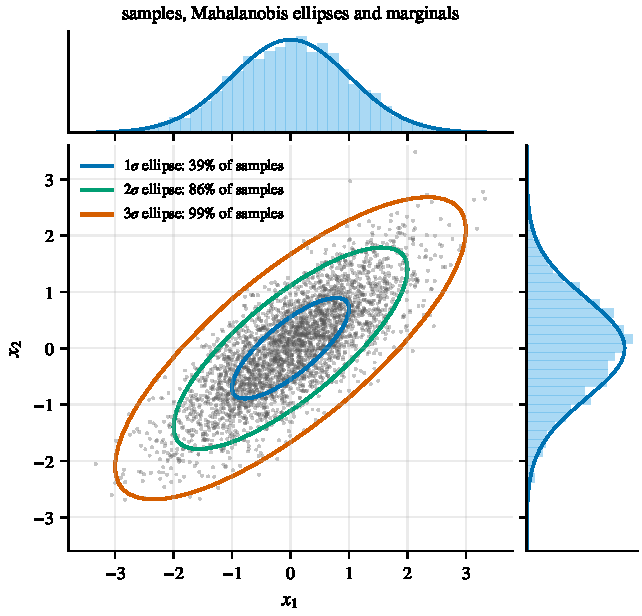
\includegraphics[width=0.92\textwidth]{fig_gauss2d.pdf}
  \caption{Samples of a correlated 2D Gaussian with the $1\sigma$, $2\sigma$ and $3\sigma$ Mahalanobis ellipses, and the two marginal densities.
  The ellipses are aligned with the eigenvectors of $\Sigma$. In two dimensions they contain 39\%, 86\% and 99\% of the probability, not
  the familiar 68--95--99.7\% of one dimension.}
  \label{fig:gauss2d}
\end{figure}

\paragraph{Geometry.} The density is constant on the ellipsoids $d_M^2(x) = c$, whose axes point along the eigenvectors of $\Sigma$ with lengths
proportional to the square roots of its eigenvalues (\cref{fig:ellipse,fig:gauss2d}). The Mahalanobis distance measures distance in units of
standard deviations along each principal axis, which makes it the natural way to ask whether a vector is ``far'' from a distribution.

\paragraph{Sampling.} To draw from $\N(\mu, \Sigma)$, factor $\Sigma = LL\T$ (Cholesky), draw $s \sim \N(0, I)$, and return $\mu + Ls$. Monte Carlo tests
of covariance propagation (Milestone 5) use exactly this.

\paragraph{Closure.} Affine maps of Gaussian vectors are Gaussian (directly from the definition). Marginals, conditionals and products of
Gaussian densities are Gaussian (next section). Hence a Gaussian belief propagated through a linear system with Gaussian noise remains
exactly Gaussian, and the Kalman filter is exact in that case. For jointly Gaussian vectors, uncorrelated implies independent: if the
covariance is block diagonal, the density factors.

\paragraph{Information form.} A Gaussian can equally be parameterized by the \term{information matrix} $\Lambda = \Sigma\inv$ and the
\emph{information vector} $\eta = \Sigma\inv\mu$. Then $-\log p(x) = \tfrac12 x\T\Lambda x - \eta\T x + \text{const}$. The information form is natural
for combining independent pieces of evidence, since their information adds, and it is the form in which optimization-based estimators work.

\subsection{Marginals and conditionals}

Partition a jointly Gaussian vector as
\begin{equation}
  \begin{bmatrix} a \\ b \end{bmatrix} \sim
  \N\!\left( \begin{bmatrix} \mu_a \\ \mu_b \end{bmatrix},
  \begin{bmatrix} \Sigma_{aa} & \Sigma_{ab} \\ \Sigma_{ba} & \Sigma_{bb} \end{bmatrix} \right),
  \qquad
  \Lambda = \Sigma\inv = \begin{bmatrix} \Lambda_{aa} & \Lambda_{ab} \\ \Lambda_{ba} & \Lambda_{bb} \end{bmatrix}.
\end{equation}

\begin{theorem}[Gaussian marginalization and conditioning]
\label{thm:gauss-cond}
\index{marginalization}\index{conditioning}
\begin{enumerate}
  \item The marginal of $a$ is $\N(\mu_a, \Sigma_{aa})$.
  \item The conditional of $a$ given $b$ is $\N(\mu_{a|b}, \Sigma_{a|b})$ with
  \begin{equation}
    \mu_{a|b} = \mu_a + \Sigma_{ab}\Sigma_{bb}\inv (b - \mu_b), \qquad
    \Sigma_{a|b} = \Sigma_{aa} - \Sigma_{ab}\Sigma_{bb}\inv\Sigma_{ba}.
    \label{eq:gauss-cond}
  \end{equation}
\end{enumerate}
\end{theorem}
\begin{proof}
The marginal follows from \cref{prop:affine} with the selection matrix $A = [I\ \ 0]$. For the conditional, define
$\tilde a = a - \Sigma_{ab}\Sigma_{bb}\inv b$. Then $\Cov(\tilde a, b) = \Sigma_{ab} - \Sigma_{ab}\Sigma_{bb}\inv\Sigma_{bb} = 0$, so $\tilde a$ and $b$ are uncorrelated,
and being jointly Gaussian they are independent. By \cref{prop:affine},
$\tilde a \sim \N(\mu_a - \Sigma_{ab}\Sigma_{bb}\inv\mu_b,\ \Sigma_{aa} - \Sigma_{ab}\Sigma_{bb}\inv\Sigma_{ba})$. Conditioning on $b$ leaves the distribution of
$\tilde a$ unchanged (independence), and $a = \tilde a + \Sigma_{ab}\Sigma_{bb}\inv b$, which gives \eqref{eq:gauss-cond}.
\end{proof}

The conditional mean moves away from $\mu_a$ in proportion to how far $b$ is from its mean, by the ``regression'' matrix $\Sigma_{ab}\Sigma_{bb}\inv$,
and the conditional covariance shrinks by a positive semi-definite amount. It does not depend on the observed value of $b$, only on the
fact that it was observed. The conditional covariance is the Schur complement $\Sigma/\Sigma_{bb}$; applying \cref{prop:block-inverse} to $\Sigma$
shows that $\Lambda_{aa} = \Sigma_{a|b}\inv$ and that the marginal information matrix is a Schur complement of $\Lambda$. The two parameterizations
therefore swap the roles of the two operations:

\begin{center}\small
\begin{tabular}{@{}lll@{}}
\toprule
 & covariance form $(\mu, \Sigma)$ & information form $(\eta, \Lambda)$ \\
\midrule
marginalize out $b$ & $\Sigma_{aa}$ \hfill(\textbf{delete rows/columns}) & $\Lambda_{aa} - \Lambda_{ab}\Lambda_{bb}\inv\Lambda_{ba}$ \hfill(Schur compl.) \\
condition on $b$ & $\Sigma_{aa} - \Sigma_{ab}\Sigma_{bb}\inv\Sigma_{ba}$ \hfill(Schur compl.) & $\Lambda_{aa}$ \hfill(\textbf{delete rows/columns}) \\
\bottomrule
\end{tabular}
\end{center}

\begin{keyidea}[marginalization is free in covariance form]
A Kalman filter stores covariances, so discarding a variable (the oldest clone of the MSCKF window) is literally deleting its rows and
columns from $P$. Optimization-based estimators store information matrices, so the same operation requires a Schur complement, which
creates fill-in and the ``marginalization prior'' of sliding-window smoothers (\cref{ch:nlls}).
\end{keyidea}

% ==============================================================================
\section{Fusing information: Bayes' rule for Gaussians}

\subsection{Combining two estimates}

Suppose two independent sensors measure the same scalar $x$, with readings $z_1 = x + n_1$ and $z_2 = x + n_2$ and noise variances $\sigma_1^2$ and
$\sigma_2^2$. With no other knowledge of $x$, the posterior density is proportional to the product of the two likelihoods,
\begin{equation}
  p(x\mid z_1, z_2) \propto \exp\!\Big(-\frac{(x - z_1)^2}{2\sigma_1^2}\Big)\exp\!\Big(-\frac{(x - z_2)^2}{2\sigma_2^2}\Big).
\end{equation}
The exponent is a quadratic in $x$; completing the square shows that the posterior is Gaussian with
\begin{equation}
  \frac{1}{\sigma^2} = \frac1{\sigma_1^2} + \frac1{\sigma_2^2}, \qquad
  \hat x = \sigma^2\Big(\frac{z_1}{\sigma_1^2} + \frac{z_2}{\sigma_2^2}\Big) = z_1 + \frac{\sigma_1^2}{\sigma_1^2 + \sigma_2^2}(z_2 - z_1).
  \label{eq:fusion}
\end{equation}
\emph{Inverse variances (information) add}, and the fused estimate is an information-weighted average. The second form already has the shape
of a Kalman update: start from $z_1$ and correct it by a gain times the discrepancy $z_2 - z_1$, with a gain between 0 and 1 that is large
when the first estimate is poor. The fused variance is smaller than both, so combining independent information always helps.

\subsection{The linear-Gaussian model}

\begin{proposition}[Linear-Gaussian posterior]
\label{prop:map-ls}
If $x \sim \N(\mu, P)$ and $z = Hx + n$ with $n \sim \N(0, R)$ independent of $x$, the posterior $p(x\mid z)$ is Gaussian, and its mean (which is
also its mode) solves the weighted least-squares problem
\begin{equation}
  \hat x = \argmin_x\ \|x - \mu\|^2_{P\inv} + \|z - Hx\|^2_{R\inv},
  \qquad \|e\|^2_{W} := e\T W e .
  \label{eq:map-ls}
\end{equation}
Its covariance is $(P\inv + H\T R\inv H)\inv$.
\end{proposition}
\begin{proof}
By Bayes' rule $p(x\mid z) \propto p(z\mid x)p(x)$, and
$-\log p(x\mid z) = \tfrac12\|x - \mu\|^2_{P\inv} + \tfrac12\|z - Hx\|^2_{R\inv} + \text{const}$. This is a convex quadratic in $x$ whose quadratic term is
$\tfrac12x\T(P\inv + H\T R\inv H)x$, so the posterior is Gaussian with that information matrix, and its mode, which for a Gaussian is the mean,
minimizes the quadratic.
\end{proof}

This is the scalar fusion rule in matrix form: the prior contributes information $P\inv$, the measurement contributes $H\T R\inv H$, and they add.
\Cref{ch:estimation} develops this into the general theory of estimators, and \cref{ch:kf} turns it into the Kalman filter.

% ==============================================================================
\section{Limit theorems and Monte Carlo}

\subsection{The law of large numbers}

Let $X_1, X_2, \dots$ be independent draws from the same distribution, with mean $\mu$ and variance $\sigma^2$, and let
$\bar X_N = \frac1N\sum_{i=1}^NX_i$ be their \term{sample mean}. Then $\E[\bar X_N] = \mu$ and, because variances of independent terms add,
$\Var(\bar X_N) = \sigma^2/N$.

\begin{theorem}[Weak law of large numbers]
\index{law of large numbers}
For every $\epsilon > 0$, $P(|\bar X_N - \mu| > \epsilon) \to 0$ as $N\to\infty$.
\end{theorem}
\begin{proof}
Chebyshev's inequality $P(|Y - \E Y| \ge \epsilon) \le \Var(Y)/\epsilon^2$ (which follows from
$\Var(Y) \ge \E[(Y - \E Y)^2\,\mathbf 1_{|Y - \E Y|\ge\epsilon}] \ge \epsilon^2P(|Y - \E Y|\ge\epsilon)$) applied to $\bar X_N$ gives the bound
$\sigma^2/(N\epsilon^2) \to 0$.
\end{proof}

The law of large numbers justifies \term{Monte Carlo} methods: to estimate an expectation, average many independent samples. The error
shrinks only like $\sigma/\sqrt N$, so each additional digit of accuracy costs a hundred times more samples.

\subsection{The central limit theorem}

\begin{theorem}[Central limit theorem]
\index{central limit theorem}
Under the same assumptions, the distribution of $\sqrt N(\bar X_N - \mu)/\sigma$ converges to $\N(0, 1)$.
\end{theorem}

\begin{figure}[t]
  \centering
  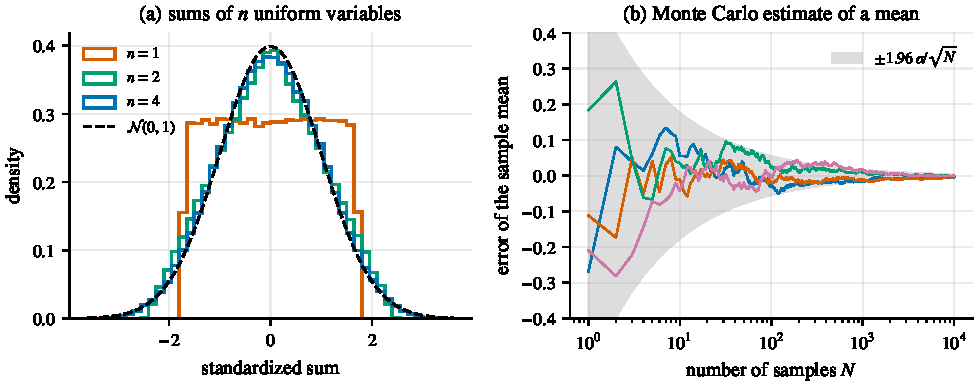
\includegraphics[width=\textwidth]{fig_clt.pdf}
  \caption{(a) The central limit theorem: histograms of the standardized sum of $n$ independent uniform variables approach the standard normal
  density already for $n = 4$. (b) Monte Carlo estimation of a mean: the error of the sample mean shrinks like $1/\sqrt N$ (gray band:
  $\pm1.96\,\sigma/\sqrt N$, the 95\% interval).}
  \label{fig:clt}
\end{figure}

Sums of many small independent effects are approximately Gaussian, whatever the distribution of each effect (\cref{fig:clt}). Electronic
sensor noise is the sum of many microscopic fluctuations, and integrating a noisy signal sums many samples; both are why Gaussian noise
models work well in navigation. They work less well for rare large errors (outliers), which is why estimators also need gating and robust
methods (\cref{ch:updates,ch:nlls}).

% ==============================================================================
\section{The chi-squared distribution}
\label{sec:chi2}

\begin{definition}
\index{chi-squared distribution}
If $s_1, \dots, s_k$ are independent standard normal variables, $\gamma = \sum_{i=1}^k s_i^2$ has the $\chi^2$ distribution with $k$ degrees of freedom,
written $\gamma \sim \chi^2_k$.
\end{definition}

\begin{proposition}[Properties of $\chi^2_k$]
$\E[\gamma] = k$ and $\Var(\gamma) = 2k$. Its density is
\begin{equation}
  p(\gamma) = \frac{\gamma^{k/2 - 1}e^{-\gamma/2}}{2^{k/2}\,\Gamma(k/2)}, \qquad \gamma > 0,
\end{equation}
where $\Gamma$ is the gamma function ($\Gamma(m) = (m - 1)!$ for integers, $\Gamma(\tfrac12) = \sqrt\pi$).
\end{proposition}
\begin{proof}[Proof of the moments and of the case $k = 1$]
For $s \sim \N(0, 1)$, $\E[s^2] = 1$ and $\E[s^4] = 3$ (integration by parts), so $\Var(s^2) = 2$; the moments of the sum follow by additivity
over independent terms. For $k = 1$, $\gamma = s^2$ takes the value $\gamma$ when $s = \pm\sqrt\gamma$, so
$p(\gamma) = 2\cdot\frac{1}{\sqrt{2\pi}}e^{-\gamma/2}\cdot\frac{\dd\sqrt\gamma}{\dd\gamma} = \frac{1}{\sqrt{2\pi\gamma}}e^{-\gamma/2}$, which is the formula with $k = 1$.
The general case follows by convolving densities (or by integrating the Gaussian density over spherical shells).
\end{proof}

\begin{theorem}[Mahalanobis distance of a Gaussian]
\label{thm:mahalanobis-chi2}
If $x \sim \N(\mu, \Sigma)$ in $\R^k$ with $\Sigma \succ 0$, then $(x-\mu)\T\Sigma\inv(x - \mu) \sim \chi^2_k$.
\end{theorem}
\begin{proof}
With $\Sigma = LL\T$, the whitened vector $s = L\inv(x - \mu)$ is $\N(0, I)$ by \cref{prop:affine}, and $(x - \mu)\T\Sigma\inv(x-\mu) = s\T s = \sum_is_i^2$.
\end{proof}

\begin{figure}[t]
  \centering
  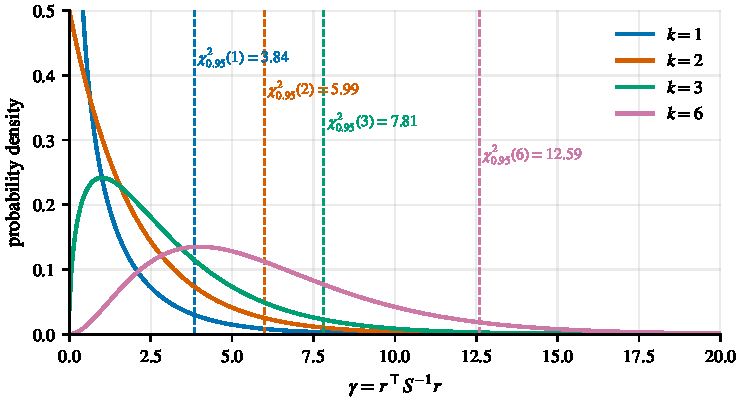
\includegraphics[width=0.84\textwidth]{fig_chi2.pdf}
  \caption{$\chi^2$ densities and their 95\% quantiles. A 2D image measurement whose normalized innovation squared exceeds $5.99$ would occur by
  chance only 5\% of the time if the filter's covariance were correct.}
  \label{fig:chi2}
\end{figure}

The \emph{quantile} $\chi^2_p(k)$ is the value below which a $\chi^2_k$ variable falls with probability $p$ (\cref{fig:chi2}; tables in
\cref{app:tables}). Because independent $\chi^2$ variables add, with their degrees of freedom adding, the sum of $N$ independent squared
Mahalanobis distances of $n$-dimensional Gaussians is $\chi^2_{Nn}$. As $k$ grows, $\chi^2_k$ is approximately $\N(k, 2k)$, so its quantiles approach
$k \pm 1.96\sqrt{2k}$.

% ==============================================================================
\section{Sample statistics and hypothesis tests}

\subsection{Estimating a mean and a variance}

Given independent samples $X_1, \dots, X_N$ of a distribution with unknown mean and variance, the natural estimates are the sample mean
$\bar X$ and the \term{sample variance}
\begin{equation}
  s^2 = \frac{1}{N - 1}\sum_{i=1}^N(X_i - \bar X)^2 .
\end{equation}
The divisor $N - 1$ makes $s^2$ unbiased. Expanding, $\sum_i(X_i - \bar X)^2 = \sum_i(X_i - \mu)^2 - N(\bar X - \mu)^2$, whose expectation is
$N\sigma^2 - N\cdot\sigma^2/N = (N - 1)\sigma^2$: one degree of freedom is used up by estimating the mean. For Gaussian samples one can show
moreover that $(N - 1)s^2/\sigma^2 \sim \chi^2_{N-1}$. This gives exact acceptance intervals for comparing a Monte Carlo sample variance with a
predicted variance, as Milestone 5 requires: the ratio $s^2/\sigma^2$ should lie between $\chi^2_{0.025}(N-1)/(N-1)$ and $\chi^2_{0.975}(N-1)/(N-1)$
95\% of the time (for $N = 500$, between $0.880$ and $1.128$; \cref{app:tables}).

\subsection{Hypothesis testing}

A \term{hypothesis test} decides whether data are compatible with a model. The recipe:
\begin{enumerate}
  \item State a \emph{null hypothesis} $H_0$, for example ``this measurement is consistent with the filter's prediction''.
  \item Choose a \emph{test statistic} whose distribution under $H_0$ is known, for example the squared Mahalanobis distance of the
        innovation, which is $\chi^2_m$ under $H_0$.
  \item Choose a \emph{significance level} $\alpha$ (often 5\%) and an \emph{acceptance region} that contains the statistic with probability
        $1 - \alpha$ under $H_0$.
  \item Reject $H_0$ if the statistic falls outside the region.
\end{enumerate}
Two errors are possible. A \emph{type I error} rejects a true $H_0$; by construction it happens with probability $\alpha$. A \emph{type II
error} accepts a false $H_0$; its probability depends on how different the truth is from $H_0$, and one minus it is the \emph{power} of the
test. Lowering $\alpha$ reduces false rejections at the price of more missed detections.

\emph{One-sided} tests reject only large values. Measurement gating is one-sided: a measurement is rejected when its Mahalanobis distance
exceeds $\chi^2_{1-\alpha}(m)$, because only large innovations indicate outliers (\cref{ch:updates}). \emph{Two-sided} tests reject both
unusually large and unusually small values. Filter consistency tests are two-sided: an average normalized error that is too small reveals an
underconfident filter just as one that is too large reveals an overconfident one (\cref{ch:consistency}).

\begin{pitfall}[a 5\% test rejects 5\% of good data]
At a 95\% gate, one in twenty perfectly good measurements is rejected. Over thousands of measurements this is expected and harmless,
provided rejections are counted. A rejection rate far from the design value is itself a symptom worth investigating.
\end{pitfall}

% ==============================================================================
\section{Nonlinear transformations}
\label{sec:linearization}

If $y = f(x)$ with $f$ nonlinear and $x \sim \N(\mu, \Sigma)$, then $y$ is generally \emph{not} Gaussian. The extended Kalman filter approximates it
by a Gaussian, linearizing $f$ about the mean:
\begin{equation}
  y \approx f(\mu) + J(x - \mu), \quad J = \frac{\partial f}{\partial x}\Big|_{\mu}
  \qquad\Longrightarrow\qquad
  y \mathrel{\dot\sim} \N\big(f(\mu),\ J\Sigma J\T\big).
\end{equation}
How much does this miss? In one dimension, Taylor expansion to second order gives
$f(x) \approx f(\mu) + f'(\mu)(x - \mu) + \tfrac12f''(\mu)(x - \mu)^2$, and taking expectations,
\begin{equation}
  \E[f(x)] \approx f(\mu) + \tfrac12f''(\mu)\,\sigma^2 .
\end{equation}
Linearization therefore ignores a \emph{bias} proportional to the curvature times the variance. The approximation is good when $f$ is nearly
linear over the region where $x$ has most of its probability mass, a few standard deviations around $\mu$.

\begin{figure}[t]
  \centering
  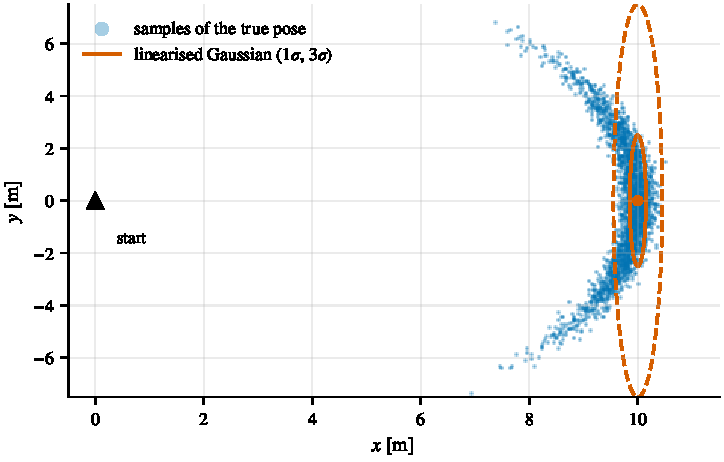
\includegraphics[width=0.84\textwidth]{fig_banana.pdf}
  \caption{A robot drives 10~m with a heading uncertainty of $\sigma_\psi = 0.25$~rad. The true distribution of its final position (samples) is a
  curved ``banana''. The linearized Gaussian (ellipses) matches its first two moments only locally, puts probability where the robot cannot be,
  and misses the curvature. Errors of this kind are why an estimator must keep its errors small, the central design principle of the
  error-state filter.}
  \label{fig:banana}
\end{figure}

\Cref{fig:banana} shows a classic failure. When heading uncertainty is large, positions are distributed along an arc, and the linearized Gaussian
is a poor description: its mean lies outside the arc, and it assigns probability to positions the robot cannot reach. Two remedies exist.
One is to reduce the uncertainty that must be linearized: the error-state filter of \cref{ch:eskf} keeps the estimation error, not the state,
as the quantity it linearizes, and continually resets it to zero. The other is to choose coordinates in which the distribution is close to
Gaussian: a Gaussian on the heading angle and travelled distance, pushed through the exact kinematics, reproduces the banana. \Cref{ch:lie}
develops that idea for rotations, and \cref{ch:nonlinear} presents a third remedy, sigma-point methods that propagate a few carefully chosen
samples instead of a linearization.

\begin{takeaways}
\begin{itemize}
  \item Bayes' rule converts a sensor model $p(z\mid x)$ and a prior $p(x)$ into the posterior $p(x\mid z)$.
  \item Affine maps propagate covariances as $A\Sigma A\T$. This single fact drives prediction, cloning and stacking.
  \item $\E[x\T Ax] = \tr(A\Sigma) + \mu\T A\mu$; the normalized squared error of an $n$-dimensional Gaussian averages to $n$.
  \item In covariance form, marginalization deletes rows and columns and conditioning takes a Schur complement. Information form is the reverse.
  \item Fusing independent Gaussian information adds inverse covariances; the result is a gain-weighted correction.
  \item Monte Carlo errors shrink like $1/\sqrt N$; sums of many small effects are nearly Gaussian.
  \item The squared Mahalanobis distance of an $n$-dimensional Gaussian is $\chi^2_n$: the basis of gating and consistency tests.
  \item Linearization ignores curvature-induced bias and fails when uncertainty is large relative to curvature.
\end{itemize}
\end{takeaways}

\begin{exercises}
  \item A gyro is either healthy (99\%) or faulty (1\%). A self-test flags 98\% of faulty units and 3\% of healthy ones. A unit is flagged; what is
        the probability that it is faulty?
  \item Let $x \sim \N(0, \diag(1, 4))$ and $y = Ax$ with $A$ a rotation by $30^\circ$. Compute $\Cov(y)$ and sketch the $1\sigma$ ellipses of $x$ and $y$.
  \item Prove that $\Sigma_{a|b} \preceq \Sigma_{aa}$: conditioning never increases uncertainty in the Loewner order. When is the inequality an equality?
  \item Derive the information-form marginal $\Lambda_{aa} - \Lambda_{ab}\Lambda_{bb}\inv\Lambda_{ba}$ from \cref{prop:block-inverse} and show that it equals $\Sigma_{aa}\inv$.
  \item Complete the square to derive \eqref{eq:fusion}.
  \item Solve \eqref{eq:map-ls} by setting the gradient to zero, and show that the solution can be written $\hat x = \mu + K(z - H\mu)$ for
        $K = (P\inv + H\T R\inv H)\inv H\T R\inv$.
  \item For $x \sim \N(0, \sigma^2)$ and $y = x^2$, compute the exact mean of $y$ and its first-order linearized prediction. Explain the discrepancy.
  \item What fraction of a 2D Gaussian's probability lies inside its $1\sigma$ Mahalanobis ellipse? (Hint: $P(\chi^2_2 \le 1)$.) Inside its $3\sigma$ ellipse?
  \item Show that $\E[s^4] = 3$ for $s \sim \N(0, 1)$ by integrating by parts.
  \item A Monte Carlo test with $N = 100$ runs finds a sample variance 25\% larger than predicted. Is this evidence of an error at the 5\% level?
\end{exercises}
% Solutions to the exercises of Chapter 5.
\begin{solutions}
  \item Let $F$ = faulty and $T$ = flagged. By the law of total probability $P(T) = 0.98\cdot0.01 + 0.03\cdot0.99 = 0.0098 + 0.0297 = 0.0395$, and by
        Bayes' rule
        \[
          P(F\mid T) = \frac{P(T\mid F)P(F)}{P(T)} = \frac{0.0098}{0.0395} = 0.248 .
        \]
        Only one flagged unit in four is actually faulty. The test is good, but faults are rare: the 3\% false-alarm rate applied to the 99\% of
        healthy units produces three times as many flags as the faulty units do. The prior matters as much as the likelihood.

  \item With $c = \cos30^\circ$ and $s = \sin30^\circ$, \cref{prop:affine} gives
        \[
          \Cov(y) = A\diag(1, 4)A\T = \begin{bmatrix} c^2 + 4s^2 & -3cs \\ -3cs & s^2 + 4c^2 \end{bmatrix}
          = \begin{bmatrix} 1.75 & -1.299 \\ -1.299 & 3.25 \end{bmatrix}.
        \]
        A rotation does not change the eigenvalues, still 1 and 4. The $1\sigma$ ellipse of $x$ has semi-axes 1 along $x_1$ and 2 along $x_2$; that
        of $y$ is the same ellipse rotated by $30^\circ$, its long axis (length 2) along $Ae_2 = (-\tfrac12, \tfrac{\sqrt3}{2})$, at $120^\circ$ from the
        first axis. The negative covariance says that $y_1$ and $y_2$ tend to have opposite signs, as the tilt of the ellipse shows.

  \item The difference is
        \[
          \Sigma_{aa} - \Sigma_{a|b} = \Sigma_{ab}\Sigma_{bb}\inv\Sigma_{ba} = \big(\Sigma_{bb}^{-1/2}\Sigma_{ba}\big)\T\big(\Sigma_{bb}^{-1/2}\Sigma_{ba}\big) \succeq 0,
        \]
        because $x\T\Sigma_{ab}\Sigma_{bb}\inv\Sigma_{ba}x = \|\Sigma_{bb}^{-1/2}\Sigma_{ba}x\|^2 \ge 0$ for every $x$ (with $\Sigma_{bb}^{-1/2}$ any square root of
        $\Sigma_{bb}\inv \succ 0$). Equality holds for all $x$ exactly when $\Sigma_{ba}x = 0$ for all $x$, i.e.\ when $\Sigma_{ab} = 0$: $a$ and $b$ are uncorrelated,
        hence (being jointly Gaussian) independent, and observing $b$ says nothing about $a$.

  \item Order the variables as $(b, a)$, so that $\Lambda$ becomes $\begin{bmatrix}\Lambda_{bb} & \Lambda_{ba}\\ \Lambda_{ab} & \Lambda_{aa}\end{bmatrix}$ and its inverse is
        $\begin{bmatrix}\Sigma_{bb} & \Sigma_{ba}\\ \Sigma_{ab} & \Sigma_{aa}\end{bmatrix}$. By \cref{prop:block-inverse}, with the top-left block $\Lambda_{bb}$ playing the
        role of $A$, the bottom-right block of the inverse is the inverse of the Schur complement:
        \[
          \Sigma_{aa} = \big(\Lambda_{aa} - \Lambda_{ab}\Lambda_{bb}\inv\Lambda_{ba}\big)\inv
          \quad\Longleftrightarrow\quad \Lambda_{aa} - \Lambda_{ab}\Lambda_{bb}\inv\Lambda_{ba} = \Sigma_{aa}\inv .
        \]
        The marginal of $a$ is $\N(\mu_a, \Sigma_{aa})$, whose information matrix is $\Sigma_{aa}\inv$: in information form, marginalization is this Schur
        complement. (The same proposition gives the marginal information vector $\eta_a - \Lambda_{ab}\Lambda_{bb}\inv\eta_b$.)

  \item Up to terms that do not involve $x$, the exponent is
        \[
          -\frac{(x - z_1)^2}{2\sigma_1^2} - \frac{(x - z_2)^2}{2\sigma_2^2}
          = -\frac12\Big(\frac{1}{\sigma_1^2} + \frac{1}{\sigma_2^2}\Big)x^2 + \Big(\frac{z_1}{\sigma_1^2} + \frac{z_2}{\sigma_2^2}\Big)x + \text{const}
          = -\frac{(x - \hat x)^2}{2\sigma^2} + \text{const},
        \]
        where matching the coefficient of $x^2$ gives $1/\sigma^2 = 1/\sigma_1^2 + 1/\sigma_2^2$ and matching that of $x$ gives
        $\hat x/\sigma^2 = z_1/\sigma_1^2 + z_2/\sigma_2^2$. A density proportional to $\exp(-(x - \hat x)^2/2\sigma^2)$ is $\N(\hat x, \sigma^2)$. Finally, with
        $\sigma^2 = \sigma_1^2\sigma_2^2/(\sigma_1^2 + \sigma_2^2)$,
        $\hat x = (\sigma_2^2z_1 + \sigma_1^2z_2)/(\sigma_1^2 + \sigma_2^2) = z_1 + \sigma_1^2(z_2 - z_1)/(\sigma_1^2 + \sigma_2^2)$, the second form of \eqref{eq:fusion}.

  \item The cost $J(x) = (x - \mu)\T P\inv(x - \mu) + (z - Hx)\T R\inv(z - Hx)$ has gradient $2P\inv(x - \mu) - 2H\T R\inv(z - Hx)$. Setting it to zero,
        \[
          \big(P\inv + H\T R\inv H\big)\hat x = P\inv\mu + H\T R\inv z .
        \]
        Write $\hat x = \mu + \delta$ and subtract $(P\inv + H\T R\inv H)\mu$ from both sides: $(P\inv + H\T R\inv H)\,\delta = H\T R\inv(z - H\mu)$, so
        $\hat x = \mu + K(z - H\mu)$ with $K = (P\inv + H\T R\inv H)\inv H\T R\inv$. The Hessian $2(P\inv + H\T R\inv H) \succ 0$ confirms a minimum. By the push-through
        identity $(P\inv + H\T R\inv H)\inv H\T R\inv = PH\T(HPH\T + R)\inv$ this is the Kalman gain of \cref{ch:kf}.

  \item Exactly, $\E[y] = \E[x^2] = \sigma^2$ (and $\Var(y) = \E[x^4] - \sigma^4 = 2\sigma^4$). Linearizing $f(x) = x^2$ at the mean $\mu = 0$ gives $f(0) = 0$ and $J = 2\mu = 0$:
        the predicted mean is $0$ and the predicted variance is $0$, a deterministic $y$. The linearization sees a function that is flat at the
        expansion point and misses the curvature entirely. The second-order correction $\tfrac12f''(\mu)\sigma^2 = \sigma^2$ of \cref{sec:linearization} accounts
        for the whole discrepancy (exactly, because $f$ is quadratic). This is the worst case for an EKF: linearizing at a stationary point of
        the measurement function.

  \item The squared Mahalanobis distance of a 2D Gaussian is $\chi^2_2$, whose density $\tfrac12e^{-\gamma/2}$ integrates to $P(\chi^2_2 \le c) = 1 - e^{-c/2}$.
        The $k\sigma$ ellipse is $d_M^2 = k^2$:
        \[
          P(1\sigma) = 1 - e^{-1/2} = 0.393, \qquad P(2\sigma) = 1 - e^{-2} = 0.865, \qquad P(3\sigma) = 1 - e^{-9/2} = 0.989 .
        \]
        Compare $0.683$, $0.954$ and $0.997$ in one dimension (and $0.199$, $0.739$, $0.971$ in three): the more dimensions, the more likely a sample lies outside
        the ``one-sigma'' region, because it must be close to the mean in every direction at once.

  \item With $\varphi(s) = e^{-s^2/2}/\sqrt{2\pi}$ we have $\varphi'(s) = -s\varphi(s)$. Integrating by parts with $u = s^3$ and $\dd v = s\varphi\,\dd s = -\dd\varphi$,
        \[
          \E[s^4] = \int_{-\infty}^{\infty}s^3\cdot s\varphi(s)\,\dd s = \big[-s^3\varphi(s)\big]_{-\infty}^{\infty} + 3\int_{-\infty}^{\infty}s^2\varphi(s)\,\dd s = 0 + 3\,\E[s^2] .
        \]
        The same step with $u = s$ gives $\E[s^2] = [-s\varphi]_{-\infty}^{\infty} + \int\varphi = 1$. Hence $\E[s^4] = 3$ and $\Var(s^2) = 3 - 1 = 2$, the variance used for $\chi^2_k$.

  \item Under the null hypothesis that the predicted variance is right, $99\,s^2/\sigma^2 \sim \chi^2_{99}$, so the ratio $s^2/\sigma^2$ lies in
        $[\chi^2_{0.025}(99), \chi^2_{0.975}(99)]/99 = [0.741, 1.297]$ with probability 95\% (\cref{app:tables}). The observed ratio $1.25$ is inside the
        interval: \emph{not} significant at the 5\% level (the two-sided $p$-value is about $0.09$). With 100 runs, a variance can be off by 25\%
        without the test noticing; the expected ratio $1.25$ would leave the interval only from about 140 runs, and a 10\% error needs
        roughly a thousand. Monte Carlo variance checks need many runs (Exercise 17.6).
\end{solutions}

